% answers.tex —— 2011 年·浙江卷·理科 · 参考答案与详细解析片段
% 由 tools/generate_projects.py 依来源总账自 2011/2011_数学真题_浙江理_试题.md + 2011/2011_数学真题_浙江理_解析正文.md + 2011/2011_数学真题_浙江理_答案要点.md 生成，勿手改（改源 MD 后重跑）

\begin{answer}
\gksolhead{1}{}

\textbf{题目}：

设函数 $f(x)=\begin{cases}-x,&x\leqslant0,\\x^2,&x>0.\end{cases}$ 若 $f(\alpha)=4$，则实数 $\alpha=$\mbox{（　　）}

（A）$-4$ 或 $-2$

（B）$-4$ 或 $2$

（C）$-2$ 或 $4$

（D）$-2$ 或 $2$

\Needspace{4\baselineskip}
\textbf{解析}
若 $\alpha\leqslant0$，$-\alpha=4$，$\alpha=-4$；若 $\alpha>0$，$\alpha^2=4$，$\alpha=2$。故 $\alpha=-4$ 或 $2$，选 B。

\gkanswer{答案：B。}

\end{answer}
\begin{answer}
\gksolhead{2}{}

\textbf{题目}：

把复数 $z$ 的共轭复数记作 $\bar z$，$\mathrm i$ 为虚数单位，若 $z=1+\mathrm i$，则 $(1+\bar z)\cdot z=$\mbox{（　　）}

（A）$3-\mathrm i$

（B）$3+\mathrm i$

（C）$1+3\mathrm i$

（D）$3$

\Needspace{4\baselineskip}
\textbf{解析}
$\bar z=1-\mathrm i$，故 $(1+\bar z)z=(2-\mathrm i)(1+\mathrm i)=3+\mathrm i$。选 B。

\gkanswer{答案：B。}

\end{answer}
\begin{answer}
\gksolhead{3}{}

\textbf{题目}：

若某几何体的三视图如图所示，则这个几何体的直观图可以是\mbox{（　　）}

（A）图 A

（B）图 B

（C）图 C

（D）图 D
\nopagebreak[4]
\begin{center}% 2011 年浙江卷理科第 3 题：三视图与四个直观图选项。
% 来源 PDF：普通高考/2011/2011浙江理.pdf，SHA-256 0239778f574bc3ce6d7aca5024aa6333f80d131abaf699f79c46472394f8cd65。
% 原页：第 1 页第 1 栏，书页码 709。示意图。
\begin{tikzpicture}[>=stealth, semithick, font=\small, scale=0.9]
  % 三视图
  \draw[thick] (0,0)--(0,1.6)--(0.9,1.6)--(0.9,0.9)--(1.6,0.9)--(1.6,0)--cycle;
  \node[below] at (0.8,-0.1) {正视图};
  \draw[thick] (2.4,0) rectangle (3.8,1.6);
  \draw[dashed] (2.4,0.9)--(3.8,0.9);
  \node[below] at (3.1,-0.1) {侧视图};
  \draw[thick] (0.2,-2.4) rectangle (1.8,-0.8);
  \draw[thick] (0.2,-0.8)--(1.8,-2.4);
  \node[below] at (1.0,-2.5) {俯视图};
  % 选项
  \begin{scope}[xshift=4.2cm, yshift=-2.4cm, scale=0.55]
    \draw[thick] (0,0)--(2,0)--(2,2)--(0,2)--cycle;
    \draw[thick] (0,2)--(0.6,2.5)--(2.6,2.5)--(2,2);
    \draw[thick] (2,0)--(2.6,0.5)--(2.6,2.5);
    \draw[thick] (0.4,1.2)--(2,1.2)--(2,2);
    \node[below] at (1,-0.3) {(A)};
  \end{scope}
  \begin{scope}[xshift=7.4cm, yshift=-2.4cm, scale=0.55]
    \draw[thick] (0,0)--(2,0)--(2,2)--(0,2)--cycle;
    \draw[thick] (0,2)--(0.6,2.5)--(2.6,2.5)--(2,2);
    \draw[thick] (2,0)--(2.6,0.5)--(2.6,2.5);
    \draw[thick] (0.5,2)--(1.0,1.2)--(1.5,2);
    \node[below] at (1,-0.3) {(B)};
  \end{scope}
  \begin{scope}[xshift=10.6cm, yshift=-2.4cm, scale=0.55]
    \draw[thick] (0,0)--(2,0)--(2,2)--(1.2,2)--(1.2,1.2)--(0,1.2)--cycle;
    \draw[thick] (0,1.2)--(0.6,1.7)--(2.6,1.7)--(2,2);
    \draw[thick] (2,0)--(2.6,0.5)--(2.6,1.7);
    \draw[thick] (1.2,2)--(1.2,1.2)--(0,1.2);
    \node[below] at (1,-0.6) {(C)};
  \end{scope}
  \begin{scope}[xshift=13.8cm, yshift=-2.4cm, scale=0.55]
    \draw[thick] (0,0)--(2,0)--(2,2)--(0,2)--cycle;
    \draw[thick] (0,2)--(0.6,2.5)--(2.6,2.5)--(2,2);
    \draw[thick] (2,0)--(2.6,0.5)--(2.6,2.5);
    \draw[thick] (0.6,0.5) rectangle (1.4,1.8);
    \node[below] at (1,-0.3) {(D)};
  \end{scope}
\end{tikzpicture}
\end{center}
\nopagebreak[4]
\Needspace{4\baselineskip}
\textbf{解析}
正视图为 L 形，说明几何体上方有一矩形缺口；俯视图为带对角线的正方形，说明缺口底面是斜面；侧视图矩形中的水平虚线正是缺口底面的投影。四个直观图中只有（C）同时具有 L 形正面与斜面缺口。选 C。

\gkanswer{答案：C。}

\end{answer}
\begin{answer}
\gksolhead{4}{}

\textbf{题目}：

下列命题中错误的是\mbox{（　　）}

（A）如果平面 $\alpha\perp$ 平面 $\beta$，那么平面 $\alpha$ 内一定存在直线平行于平面 $\beta$

（B）如果平面 $\alpha$ 不垂直于平面 $\beta$，那么平面 $\alpha$ 内一定不存在直线垂直于平面 $\beta$

（C）如果平面 $\alpha\perp$ 平面 $\gamma$，平面 $\beta\perp$ 平面 $\gamma$，$\alpha\cap\beta=l$，那么 $l\perp$ 平面 $\gamma$

（D）如果平面 $\alpha\perp$ 平面 $\beta$，那么平面 $\alpha$ 内所有直线都垂直于平面 $\beta$

\Needspace{4\baselineskip}
\textbf{解析}
（D）错误：两平面垂直时，一个平面内只有垂直于交线的直线才垂直于另一个平面，并非所有直线。（A）（B）（C）均为真命题。选 D。

\gkanswer{答案：D。}

\end{answer}
\begin{answer}
\gksolhead{5}{}

\textbf{题目}：

设实数 $x$，$y$ 满足不等式组 $\begin{cases}x+2y-5>0,\\2x+y-7>0,\\x\geqslant0,\ y\geqslant0.\end{cases}$ 若 $x$，$y$ 为整数，则 $3x+4y$ 的最小值是\mbox{（　　）}

（A）$14$

（B）$16$

（C）$17$

（D）$19$

\Needspace{4\baselineskip}
\textbf{解析}
枚举整数点：$(4,1)$ 满足 $4+2-5=1>0$、$8+1-7=2>0$，此时 $3x+4y=16$；$(3,2)$ 得 $17$，$(5,1)$ 得 $19$，其余可行点更大。故最小值为 $16$。选 B。

\gkanswer{答案：B。}

\end{answer}
\begin{answer}
\gksolhead{6}{}

\textbf{题目}：

若 $0<\alpha<\dfrac\pi2$，$-\dfrac\pi2<\beta<0$，$\cos\left(\dfrac\pi4+\alpha\right)=\dfrac13$，$\cos\left(\dfrac\pi4-\dfrac\beta2\right)=\dfrac{\sqrt3}3$，则 $\cos\left(\alpha+\dfrac\beta2\right)=$\mbox{（　　）}

（A）$\dfrac{\sqrt3}3$

（B）$-\dfrac{\sqrt3}3$

（C）$\dfrac{5\sqrt3}9$

（D）$-\dfrac{\sqrt6}9$

\Needspace{4\baselineskip}
\textbf{解析}
\Needspace{5\baselineskip}
令 $A=\dfrac\pi4+\alpha$，$B=\dfrac\pi4-\dfrac\beta2$，则 $A\in\left(\dfrac\pi4,\dfrac{3\pi}4\right)$，$B\in\left(\dfrac\pi4,\dfrac\pi2\right)$，且
\nopagebreak[4]
\[\cos A=\frac13,\quad \sin A=\frac{2\sqrt2}3;\qquad \cos B=\frac{\sqrt3}3,\quad \sin B=\frac{\sqrt6}3.\]
\Needspace{5\baselineskip}
而 $\alpha+\dfrac\beta2=A-B$，故
\nopagebreak[4]
\[\cos(A-B)=\frac13\cdot\frac{\sqrt3}3+\frac{2\sqrt2}3\cdot\frac{\sqrt6}3=\frac{\sqrt3}9+\frac{4\sqrt3}9=\frac{5\sqrt3}9.\]
选 C。

\gkanswer{答案：C。}

\end{answer}
\begin{answer}
\gksolhead{7}{}

\textbf{题目}：

若 $a$，$b$ 为实数，则“$0<ab<1$”是“$a<\dfrac1b$ 或 $b>\dfrac1a$”的\mbox{（　　）}

（A）充分而不必要条件

（B）必要而不充分条件

（C）充分必要条件

（D）既不充分也不必要条件

\Needspace{4\baselineskip}
\textbf{解析}
若 $0<ab<1$：当 $a,b>0$ 时 $a<\dfrac1b$；当 $a,b<0$ 时 $b>\dfrac1a$。故条件充分。
反之取 $a=1,b=2$，则 $b>\dfrac1a$ 成立而 $ab=2>1$，故不必要。选 A。

\gkanswer{答案：A。}

\end{answer}
\begin{answer}
\gksolhead{8}{}

\textbf{题目}：

已知椭圆 $C_1:\dfrac{x^2}{a^2}+\dfrac{y^2}{b^2}=1$（$a>b>0$）与双曲线 $C_2:x^2-\dfrac{y^2}{4}=1$ 有公共的焦点，$C_2$ 的一条渐近线与以 $C_1$ 的长轴为直径的圆相交于 $A$，$B$ 两点。若 $C_1$ 恰好将线段 $AB$ 三等分，则\mbox{（　　）}

（A）$a^2=\dfrac{13}2$

（B）$a^2=13$

（C）$b^2=\dfrac12$

（D）$b^2=2$

\Needspace{4\baselineskip}
\textbf{解析}
双曲线 $x^2-\dfrac{y^2}4=1$ 的 $c^2=5$，故椭圆 $a^2-b^2=5$。渐近线 $y=2x$ 与圆 $x^2+y^2=a^2$ 交于 $A$、$B$，$AB$ 为直径，长 $2a$。
\Needspace{5\baselineskip}
椭圆与该直线的交点满足
\nopagebreak[4]
\[\frac{x^2}{a^2}+\frac{4x^2}{b^2}=1\Longrightarrow x^2=\frac{a^2b^2}{b^2+4a^2}.\]
\Needspace{5\baselineskip}
椭圆将 $AB$ 三等分，即椭圆截得的弦长为 $\dfrac{2a}3$。该弦两端到圆心距离为 $\dfrac a3$，而直线上点 $(x,2x)$ 到圆心距离为 $\sqrt5|x|$，故
\nopagebreak[4]
\[\sqrt5\,|x|=\frac a3\Longrightarrow x^2=\frac{a^2}{45}.\]
\Needspace{5\baselineskip}
于是
\nopagebreak[4]
\[\frac{b^2}{b^2+4a^2}=\frac1{45}\Longrightarrow45b^2=b^2+4a^2\Longrightarrow a^2=11b^2.\]
结合 $a^2-b^2=5$ 得 $b^2=\dfrac12$，$a^2=\dfrac{11}2$。选 C。

\gkanswer{答案：C。}

\end{answer}
\begin{answer}
\gksolhead{9}{}

\textbf{题目}：

有 $5$ 本不同的书，其中语文书 $2$ 本，数学书 $2$ 本，物理书 $1$ 本。若将其随机地抽取并排摆放在书架的同一层上，则同一科目的书都不相邻的概率为\mbox{（　　）}

（A）$\dfrac15$

（B）$\dfrac25$

（C）$\dfrac35$

（D）$\dfrac45$

\Needspace{4\baselineskip}
\textbf{解析}
\Needspace{5\baselineskip}
总排法 $5!=120$。记语文书相邻为 $A$，数学书相邻为 $B$：$|A|=|B|=4!\times2=48$，$|A\cap B|=3!\times2\times2=24$。故同一科目都不相邻的排法
\nopagebreak[4]
\[120-48-48+24=48,\]
概率 $\dfrac{48}{120}=\dfrac25$。选 B。

\gkanswer{答案：B。}

\end{answer}
\begin{answer}
\gksolhead{10}{}

\textbf{题目}：

设 $a$，$b$，$c$ 为实数，$f(x)=(x+a)(x^2+bx+c)$，$g(x)=(ax+1)(cx^2+bx+1)$。记集合 $S=\{x\mid f(x)=0,\ x\in\mathbf R\}$，$T=\{x\mid g(x)=0,\ x\in\mathbf R\}$，若 $|S|$，$|T|$ 分别为集合 $S$，$T$ 的元素个数，则下列结论不可能的是\mbox{（　　）}

（A）$|S|=1$ 且 $|T|=0$

（B）$|S|=1$ 且 $|T|=1$

（C）$|S|=2$ 且 $|T|=2$

（D）$|S|=2$ 且 $|T|=3$

\Needspace{4\baselineskip}
\textbf{解析}
（D）不可能。$|S|=2$ 时，$f$ 的根只有两种情形：$x=-a$ 是二重根，或 $-a$ 与二次式的某一根重合。逐一代入 $g$ 可验证 $T$ 的元素个数只能为 $0,1,2$，不可能为 $3$。（A）（B）（C）均有实例。选 D。

\gkanswer{答案：D。}

\end{answer}
\begin{answer}
\gksolhead{11}{}

\textbf{题目}：

若函数 $f(x)=x^2-|x+a|$ 为偶函数，则实数 $a=$ $\underline{\qquad}$。

\Needspace{4\baselineskip}
\textbf{解析}
\Needspace{5\baselineskip}
$f$ 为偶函数，故 $f(-x)=f(x)$：
\nopagebreak[4]
\[x^2-|{-x+a}|=x^2-|x+a|\Longrightarrow|{x-a}|=|{x+a}|\]
对任意 $x$ 成立，故 $a=0$。

\gkanswer{答案：$0$。}

\end{answer}
\begin{answer}
\gksolhead{12}{}

\textbf{题目}：

某程序框图如图所示，则该程序运行后输出的 $k$ 的值是 $\underline{\qquad}$。
\nopagebreak[4]
\begin{center}% 2011 年浙江卷理科第 12 题：程序框图。
% 来源 PDF：普通高考/2011/2011浙江理.pdf，SHA-256 0239778f574bc3ce6d7aca5024aa6333f80d131abaf699f79c46472394f8cd65。
% 原页：第 1 页第 2 栏中部，书页码 709。
\begin{tikzpicture}[>=stealth, semithick, font=\small]
  \node[draw, rounded corners=0.12cm, minimum width=1.2cm, minimum height=0.5cm] (start) at (0,0) {开始};
  \node[draw, minimum width=1.4cm, minimum height=0.5cm] (k2) at (0,-1.1) {$k=2$};
  \node[draw, minimum width=1.8cm, minimum height=0.5cm] (inc) at (0,-2.2) {$k=k+1$};
  \node[draw, minimum width=1.8cm, minimum height=0.5cm] (a) at (0,-3.3) {$a=4^k$};
  \node[draw, minimum width=1.8cm, minimum height=0.5cm] (b) at (0,-4.4) {$b=k^4$};
  \node[draw, diamond, aspect=1.7, minimum width=1.6cm, minimum height=0.9cm] (test) at (0,-5.8) {$a>b$};
  \node[draw, trapezium, trapezium left angle=72, trapezium right angle=108,
        minimum width=1.6cm, minimum height=0.55cm] (out) at (0,-7.2) {输出 $k$};
  \node[draw, rounded corners=0.12cm, minimum width=1.2cm, minimum height=0.5cm] (stop) at (0,-8.4) {结束};
  \draw[->] (start.south)--(k2.north);
  \draw[->] (k2.south)--(inc.north);
  \draw[->] (inc.south)--(a.north);
  \draw[->] (a.south)--(b.north);
  \draw[->] (b.south)--(test.north);
  \draw[->] (test.south)--(out.north) node[midway, right] {是};
  \draw[->] (out.south)--(stop.north);
  \draw[->] (test.east) -- ++(1.4,0) |- (inc.east) node[pos=0.25, right] {否};
\end{tikzpicture}
\end{center}
\nopagebreak[4]
\Needspace{4\baselineskip}
\textbf{解析}
$k=2$ 时进入循环：$k=3$，$a=4^3=64$，$b=3^4=81$，$a>b$ 不成立；$k=4$，$a=256$，$b=256$，仍不成立；$k=5$，$a=1024$，$b=625$，$a>b$ 成立，输出 $k=5$。

\gkanswer{答案：$5$。}

\end{answer}
\begin{answer}
\gksolhead{13}{}

\textbf{题目}：

设二项式 $\left(x-\dfrac{a}{\sqrt x}\right)^6$（$a>0$）的展开式中 $x^3$ 的系数为 $A$，常数项为 $B$。若 $B=4A$，则 $a$ 的值是 $\underline{\qquad}$。

\Needspace{4\baselineskip}
\textbf{解析}
\Needspace{5\baselineskip}
通项
\nopagebreak[4]
\[\mathrm C_6^k x^{6-k}\left(-\frac a{\sqrt x}\right)^k=\mathrm C_6^k(-a)^k x^{6-\frac{3k}2}.\]
\Needspace{5\baselineskip}
$x^3$ 项：$6-\dfrac{3k}2=3$，$k=2$，$A=15a^2$；常数项：$k=4$，$B=15a^4$。由 $B=4A$：
\nopagebreak[4]
\[15a^4=60a^2\Longrightarrow a^2=4\Longrightarrow a=2\ (a>0).\]

\gkanswer{答案：$2$。}

\end{answer}
\begin{answer}
\gksolhead{14}{}

\textbf{题目}：

若平面向量 $\boldsymbol\alpha$、$\boldsymbol\beta$ 满足 $|\boldsymbol\alpha|=1$，$|\boldsymbol\beta|\leqslant1$，且以向量 $\boldsymbol\alpha$、$\boldsymbol\beta$ 为邻边的平行四边形的面积为 $\dfrac12$，则 $\boldsymbol\alpha$ 和 $\boldsymbol\beta$ 的夹角 $\theta$ 的取值范围是 $\underline{\qquad}$。

\Needspace{4\baselineskip}
\textbf{解析}
\Needspace{5\baselineskip}
平行四边形面积
\nopagebreak[4]
\[S=|\boldsymbol\alpha||\boldsymbol\beta|\sin\theta=|\boldsymbol\beta|\sin\theta=\frac12.\]
\Needspace{5\baselineskip}
故 $\sin\theta=\dfrac1{2|\boldsymbol\beta|}\geqslant\dfrac12$（因 $|\boldsymbol\beta|\leqslant1$），从而
\nopagebreak[4]
\[\theta\in\left[\frac\pi6,\frac{5\pi}6\right].\]

\gkanswer{答案：$\left[\dfrac\pi6,\dfrac{5\pi}6\right]$。}

\end{answer}
\begin{answer}
\gksolhead{15}{}

\textbf{题目}：

某毕业生参加人才招聘会，分别向甲、乙、丙三个公司投递了个人简历，假定该毕业生得到甲公司面试的概率为 $\dfrac23$，得到乙、丙公司面试的概率均为 $p$，且三个公司是否让其面试是相互独立的。记 $X$ 为该毕业生得到面试的公司个数。若 $P(X=0)=\dfrac1{12}$，则随机变量 $X$ 的数学期望 $E(X)=$ $\underline{\qquad}$。

\Needspace{4\baselineskip}
\textbf{解析}
$P(X=0)=\left(1-\dfrac23\right)(1-p)^2=\dfrac13(1-p)^2=\dfrac1{12}$，故 $(1-p)^2=\dfrac14$，$p=\dfrac12$（$p\leqslant1$）。
\Needspace{5\baselineskip}
$X$ 为三个独立 0-1 变量之和，期望
\nopagebreak[4]
\[E(X)=\frac23+\frac12+\frac12=\frac53.\]

\gkanswer{答案：$\dfrac53$。}

\end{answer}
\begin{answer}
\gksolhead{16}{}

\textbf{题目}：

设 $x$，$y$ 为实数，若 $4x^2+y^2+xy=1$，则 $2x+y$ 的最大值是 $\underline{\qquad}$。

\Needspace{4\baselineskip}
\textbf{解析}
\Needspace{5\baselineskip}
令 $t=2x+y$，则 $y=t-2x$。代入 $4x^2+y^2+xy=1$：
\nopagebreak[4]
\[4x^2+(t-2x)^2+x(t-2x)=1\Longrightarrow6x^2-3tx+t^2-1=0.\]
\Needspace{5\baselineskip}
关于 $x$ 的方程有实根，判别式
\nopagebreak[4]
\[\Delta=9t^2-24(t^2-1)\geqslant0\Longrightarrow15t^2\leqslant24\Longrightarrow t\leqslant\frac{2\sqrt{10}}5.\]

\gkanswer{答案：$\dfrac{2\sqrt{10}}5$。}

\end{answer}
\begin{answer}
\gksolhead{17}{}

\textbf{题目}：

设 $F_1$，$F_2$ 分别为椭圆 $\dfrac{x^2}3+y^2=1$ 的焦点，点 $A$，$B$ 在椭圆上。若 $\overrightarrow{F_1A}=5\overrightarrow{F_2B}$，则点 $A$ 的坐标是 $\underline{\qquad}$。

\Needspace{4\baselineskip}
\textbf{解析}
\Needspace{5\baselineskip}
椭圆 $\dfrac{x^2}3+y^2=1$ 的 $c^2=2$，$F_1(-\sqrt2,0)$，$F_2(\sqrt2,0)$。设 $A(x_1,y_1)$，$B(x_2,y_2)$，由 $\overrightarrow{F_1A}=5\overrightarrow{F_2B}$：
\nopagebreak[4]
\[x_1+\sqrt2=5(x_2-\sqrt2),\qquad y_1=5y_2.\]
取 $A(0,1)$，则 $x_2=\dfrac{6\sqrt2}5$，$y_2=\dfrac15$，代入椭圆：$\dfrac{72/25}3+\dfrac1{25}=\dfrac{24}{25}+\dfrac1{25}=1$，成立。由对称性 $A(0,-1)$ 也成立。故 $A(0,\pm1)$。

\gkanswer{答案：$(0,\pm1)$。}

\end{answer}
\begin{answer}
\gksolhead{18}{}

\textbf{题目}：

在 $\triangle ABC$ 中，角 $A$，$B$，$C$ 所对的边分别为 $a$，$b$，$c$。已知 $\sin A+\sin C=p\sin B$（$p\in\mathbf R$），且 $ac=\dfrac14b^2$。

（1） 当 $p=\dfrac54$，$b=1$ 时，求 $a$，$c$ 的值；

（2） 若角 $B$ 为锐角，求 $p$ 的取值范围。

\Needspace{4\baselineskip}
\textbf{解析}
\gksubpart{(1)}
由正弦定理 $a+c=pb=\dfrac54$（$b=1$），又 $ac=\dfrac14$。故 $a,c$ 是方程 $t^2-\dfrac54t+\dfrac14=0$ 的两根，解得 $t=1,\dfrac14$。故 $(a,c)=\left(1,\dfrac14\right)$ 或 $\left(\dfrac14,1\right)$。

\gksubpart{(2)}
\Needspace{5\baselineskip}
由余弦定理
\nopagebreak[4]
\[b^2=a^2+c^2-2ac\cos B=(a+c)^2-2ac(1+\cos B).\]
\Needspace{5\baselineskip}
代入 $a+c=pb$、$ac=\dfrac14b^2$：
\nopagebreak[4]
\[b^2=p^2b^2-\frac12b^2(1+\cos B)\Longrightarrow p^2=\frac{3+\cos B}2.\]
$B$ 为锐角，$0<\cos B<1$，故 $\dfrac32<p^2<2$，即 $p\in\left(\dfrac{\sqrt6}2,\sqrt2\right)$。

\gkanswer{答案（1）：$a=1$，$c=\dfrac14$ 或 $a=\dfrac14$，$c=1$。}

\gkanswer{答案（2）：$\left(\dfrac{\sqrt6}2,\sqrt2\right)$。}

\end{answer}
\begin{answer}
\gksolhead{19}{}

\textbf{题目}：

已知公差不为 $0$ 的等差数列 $\{a_n\}$ 的首项 $a_1$ 为 $a$（$a\in\mathbf R$）。设数列的前 $n$ 项和为 $S_n$，且 $\dfrac1{a_1}$，$\dfrac1{a_2}$，$\dfrac1{a_4}$ 成等比数列。

（1） 求数列 $\{a_n\}$ 的通项公式及 $S_n$；

（2） 记 $A_n=\dfrac1{S_1}+\dfrac1{S_2}+\dfrac1{S_3}+\cdots+\dfrac1{S_n}$，$B_n=\dfrac1{a_1}+\dfrac1{a_2}+\dfrac1{a_{2^2}}+\cdots+\dfrac1{a_{2^{n-1}}}$。当 $n\geqslant2$ 时，试比较 $A_n$ 与 $B_n$ 的大小。

\Needspace{4\baselineskip}
\textbf{解析}
\gksubpart{(1)}
\Needspace{5\baselineskip}
$\dfrac1{a_1},\dfrac1{a_2},\dfrac1{a_4}$ 成等比，故 $a_2^2=a_1a_4$。设公差 $d\neq0$：
\nopagebreak[4]
\[(a+d)^2=a(a+3d)\Longrightarrow d^2=ad\Longrightarrow d=a.\]
故 $a_n=a+(n-1)a=na$，$S_n=\dfrac{a n(n+1)}2$。

\gksubpart{(2)}
\nopagebreak[4]
\[A_n=\sum_{k=1}^n\frac{2}{ak(k+1)}=\frac2a\left(1-\frac1{n+1}\right)=\frac{2n}{a(n+1)},\]
\nopagebreak[4]
\[B_n=\sum_{k=1}^n\frac1{a2^{k-1}}=\frac1a\cdot\frac{1-2^{-n}}{1-\frac12}=\frac2a(1-2^{-n}).\]
\Needspace{5\baselineskip}
当 $n\geqslant2$ 时，
\nopagebreak[4]
\[\frac{2n}{n+1}=2-\frac2{n+1}<2-2^{1-n}=\frac{2(2^n-1)}{2^n},\]
因为 $\dfrac2{n+1}>2^{1-n}$。故 $A_n<B_n$。

\gkanswer{答案（1）：$a_n=na$，$S_n=\dfrac{a n(n+1)}2$。}

\gkanswer{答案（2）：$A_n<B_n$。}

\end{answer}
\begin{answer}
\gksolhead{20}{}

\textbf{题目}：

如图，在三棱锥 $P-ABC$ 中，$AB=AC$，$D$ 为 $BC$ 的中点，$PO\perp$ 平面 $ABC$，垂足 $O$ 落在线段 $AD$ 上，已知 $BC=8$，$PO=4$，$AO=3$，$OD=2$。

（1） 证明：$AP\perp BC$；

（2） 在线段 $AP$ 上是否存在点 $M$，使得二面角 $A-MC-B$ 为直二面角？若存在，求出 $AM$ 的长；若不存在，请说明理由。
\nopagebreak[4]
\begin{center}% 2011 年浙江卷理科第 20 题：三棱锥 P-ABC，O 在 AD 上，PO⊥平面 ABC。
% 来源 PDF：普通高考/2011/2011浙江理.pdf，SHA-256 0239778f574bc3ce6d7aca5024aa6333f80d131abaf699f79c46472394f8cd65。
% 原页：第 2 页第 1 栏，书页码 710。示意。
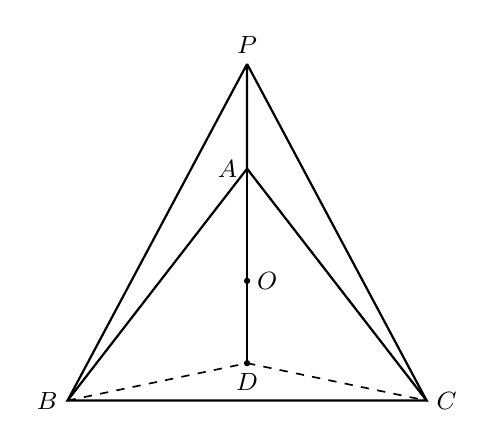
\begin{tikzpicture}[>=stealth, semithick, font=\small, scale=0.95]
  \coordinate (D) at (0,0);
  \coordinate (B) at (-2.4,-0.5);
  \coordinate (C) at (2.4,-0.5);
  \coordinate (A) at (0,2.6);
  \coordinate (O) at (0,1.1);
  \coordinate (P) at (0,4.0);
  \draw[thick] (A)--(B)--(C)--cycle;
  \draw[thick] (P)--(A) (P)--(B) (P)--(C);
  \draw[dashed] (A)--(C);
  \draw[dashed] (P)--(O);
  \draw[dashed] (B)--(D);
  \draw[dashed] (D)--(C);
  \draw (A)--(D);
  \fill (D) circle (1.2pt) node[below] {$D$};
  \fill (O) circle (1.2pt) node[right] {$O$};
  \node[left] at (A) {$A$};
  \node[left] at (B) {$B$};
  \node[right] at (C) {$C$};
  \node[above] at (P) {$P$};
\end{tikzpicture}
\end{center}
\nopagebreak[4]
\Needspace{4\baselineskip}
\textbf{解析}
\gksubpart{(1)}
由 $AB=AC$、$D$ 为 $BC$ 中点得 $AD\perp BC$。又 $PO\perp$ 平面 $ABC$，故 $PO\perp BC$。$BC\perp AD$ 且 $BC\perp PO$，而 $AD$、$PO$ 是平面 $PAD$ 内两条相交直线，故 $BC\perp$ 平面 $PAD$，从而 $BC\perp AP$。

\gksubpart{(2)}
\Needspace{5\baselineskip}
以 $D$ 为原点，$DB$ 为 $x$ 轴、$DA$ 为 $y$ 轴、过 $D$ 且平行 $OP$ 的方向为 $z$ 轴建立坐标系：
\nopagebreak[4]
\[D(0,0,0),\ B(4,0,0),\ C(-4,0,0),\ A(0,-5,0),\ O(0,-2,0),\ P(0,-2,4).\]
\Needspace{5\baselineskip}
设 $M=A+t\overrightarrow{AP}=(0,-5+3t,4t)$（$0\leqslant t\leqslant1$）。平面 $AMC$ 与 $BMC$ 的法向量分别为
\nopagebreak[4]
\[\boldsymbol n_1=\overrightarrow{MC}\times\overrightarrow{MA},\qquad \boldsymbol n_2=\overrightarrow{MC}\times\overrightarrow{MB}.\]
\Needspace{5\baselineskip}
计算并令 $\boldsymbol n_1\cdot\boldsymbol n_2=0$，化简得
\nopagebreak[4]
\[t(5t-3)=0.\]
\Needspace{5\baselineskip}
$t=0$ 时 $M=A$，二面角退化；故 $t=\dfrac35$。此时
\nopagebreak[4]
\[AM=t\cdot AP=\frac35\sqrt{0^2+3^2+4^2}=3.\]
故存在点 $M$，且 $AM=3$。

\gkanswer{答案（1）：证明见解析。}

\gkanswer{答案（2）：存在，$AM=3$。}

\end{answer}
\begin{answer}
\gksolhead{21}{}

\textbf{题目}：

已知抛物线 $C_1:x^2=y$，圆 $C_2:x^2+(y-4)^2=1$ 的圆心为点 $M$。

（1） 求点 $M$ 到抛物线 $C_1$ 的准线的距离；

（2） 已知点 $P$ 是抛物线 $C_1$ 上一点（异于原点），过点 $P$ 作圆 $C_2$ 的两条切线，交抛物线 $C_1$ 于 $A$，$B$ 两点，若过 $M$，$P$ 两点的直线 $l$ 垂直于 $AB$，求直线 $l$ 的方程。
\nopagebreak[4]
\begin{center}% 2011 年浙江卷理科第 21 题：抛物线 C1: x^2=y 与圆 C2: x^2+(y-4)^2=1。
% 来源 PDF：普通高考/2011/2011浙江理.pdf，SHA-256 0239778f574bc3ce6d7aca5024aa6333f80d131abaf699f79c46472394f8cd65。
% 原页：第 2 页第 2 栏，书页码 710。示意。
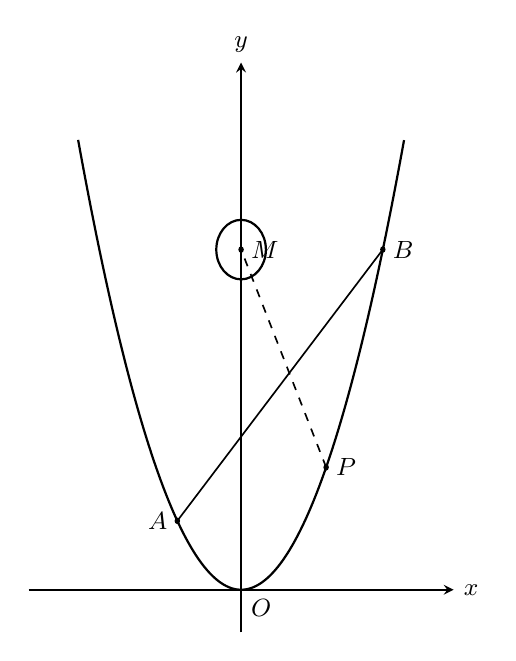
\begin{tikzpicture}[>=stealth, semithick, font=\small, scale=0.9, yscale=1.2]
  \draw[->] (-3,0)--(3,0) node[right] {$x$};
  \draw[->] (0,-0.5)--(0,6.2) node[above] {$y$};
  \draw[thick, domain=-2.3:2.3, samples=120] plot (\x, {\x*\x});
  \draw[thick] (0,4) circle (0.35);
  \fill (0,4) circle (1.1pt) node[right] {$M$};
  \coordinate (P) at (1.2,1.44);
  \fill (P) circle (1.1pt) node[right] {$P$};
  \coordinate (A) at (-0.9,0.81);
  \coordinate (B) at (2.0,4.0);
  \fill (A) circle (1.1pt) node[left] {$A$};
  \fill (B) circle (1.1pt) node[right] {$B$};
  \draw (A)--(B);
  \draw[dashed] (P)--(0,4);
  \node[below right] at (0,0) {$O$};
\end{tikzpicture}
\end{center}
\nopagebreak[4]
\Needspace{4\baselineskip}
\textbf{解析}
\gksubpart{(1)}
抛物线 $x^2=y$ 的准线为 $y=-\dfrac14$，圆心 $M(0,4)$ 到准线距离为 $4+\dfrac14=\dfrac{17}4$。

\gksubpart{(2)}
\Needspace{5\baselineskip}
设 $P(t,t^2)$（$t\neq0$）。过 $P$ 的直线 $y-t^2=m(x-t)$ 与圆相切，圆心到直线距离为 $1$：
\nopagebreak[4]
\[(t^2-4-mt)^2=m^2+1.\]
\Needspace{5\baselineskip}
整理为关于 $m$ 的二次方程
\nopagebreak[4]
\[(t^2-1)m^2-2t(t^2-4)m+(t^2-4)^2-1=0,\]
\Needspace{5\baselineskip}
两切线斜率 $m_1,m_2$ 满足
\nopagebreak[4]
\[m_1+m_2=\frac{2t(t^2-4)}{t^2-1}.\]
\Needspace{5\baselineskip}
切线与抛物线另一交点横坐标为 $m-t$，故
\nopagebreak[4]
\[k_{AB}=(m_1-t)+(m_2-t)=m_1+m_2-2t.\]
\Needspace{5\baselineskip}
由 $MP\perp AB$，$k_{MP}=\dfrac{t^2-4}{t}$，故 $k_{AB}=-\dfrac{t}{t^2-4}$。代入得
\nopagebreak[4]
\[\frac{2t(t^2-4)}{t^2-1}-2t=-\frac{t}{t^2-4}.\]
\Needspace{5\baselineskip}
$t\neq0$，化简：
\nopagebreak[4]
\[\frac{-6}{t^2-1}=\frac1{4-t^2}\Longrightarrow t^2=\frac{23}5.\]
\Needspace{5\baselineskip}
直线 $l$ 过 $M(0,4)$、$P(t,t^2)$，斜率 $\dfrac{t^2-4}{t}=\dfrac{3}{5t}$，故
\nopagebreak[4]
\[y=4+\frac{3}{5t}x.\]
\Needspace{5\baselineskip}
由 $t=\pm\dfrac{\sqrt{115}}5$，得
\nopagebreak[4]
\[y=4\pm\frac{3\sqrt{115}}{115}x.\]

\gkanswer{答案（1）：$\dfrac{17}4$。}

\gkanswer{答案（2）：$y=4\pm\dfrac{3\sqrt{115}}{115}x$。}

\end{answer}
\begin{answer}
\gksolhead{22}{}

\textbf{题目}：

设函数 $f(x)=(x-a)^2\ln x$，$a\in\mathbf R$。

（1） 若 $x=\mathrm e$ 为 $y=f(x)$ 的极值点，求实数 $a$；

（2） 求实数 $a$ 的取值范围，使得对任意的 $x\in(0,3\mathrm e]$，恒有 $f(x)\leqslant4\mathrm e^2$ 成立。

注：$\mathrm e$ 为自然对数的底数。

\Needspace{4\baselineskip}
\textbf{解析}
\gksubpart{(1)}
\nopagebreak[4]
\[f'(x)=2(x-a)\ln x+\frac{(x-a)^2}{x}.\]
\Needspace{5\baselineskip}
$x=\mathrm e$ 为极值点，故 $f'(\mathrm e)=0$：
\nopagebreak[4]
\[(\mathrm e-a)\left[2+\frac{\mathrm e-a}{\mathrm e}\right]=0\Longrightarrow a=\mathrm e\ \text{\text{或}}\ a=3\mathrm e.\]
$a=3\mathrm e$ 时 $f'$ 在 $x=\mathrm e$ 两侧不变号，不是极值点；$a=\mathrm e$ 时变号。故 $a=\mathrm e$。

\gksubpart{(2)}
\Needspace{5\baselineskip}
$x\in(0,1]$ 时 $\ln x\leqslant0$，$f(x)\leqslant0<4\mathrm e^2$，自动成立。只需考察 $x\in(1,3\mathrm e]$。此时 $\ln x>0$，条件等价于
\nopagebreak[4]
\[|x-a|\leqslant\frac{2\mathrm e}{\sqrt{\ln x}}\quad(1<x\leqslant3\mathrm e).\]
\Needspace{5\baselineskip}
即对每个 $x$，
\nopagebreak[4]
\[a\in\left[x-\frac{2\mathrm e}{\sqrt{\ln x}},\ x+\frac{2\mathrm e}{\sqrt{\ln x}}\right].\]
\Needspace{5\baselineskip}
记 $g_1(x)=x-\dfrac{2\mathrm e}{\sqrt{\ln x}}$，$g_2(x)=x+\dfrac{2\mathrm e}{\sqrt{\ln x}}$。$g_1$ 在 $(1,3\mathrm e]$ 上递增，最大值为 $g_1(3\mathrm e)=3\mathrm e-\dfrac{2\mathrm e}{\sqrt{1+\ln3}}$；$g_2$ 的最小值在 $x=\mathrm e$ 取得，为 $g_2(\mathrm e)=3\mathrm e$。故所求范围为
\nopagebreak[4]
\[\left[3\mathrm e-\frac{2\mathrm e}{\sqrt{1+\ln3}},\ 3\mathrm e\right].\]

\gkanswer{答案（1）：$a=\mathrm e$。}

\gkanswer{答案（2）：$\left[3\mathrm e-\dfrac{2\mathrm e}{\sqrt{1+\ln3}},\,3\mathrm e\right]$。}

\end{answer}